%%%%%%%%%%%%%%%%%%%%%%%%%%%%%%%%%%%%%%%%%%%%%%%%%%%%%%%%%%%%%%%%%%%%%
%
% CSCI 1430 Written Question Template
%
% This is a LaTeX document. LaTeX is a markup language for producing
% documents. Your task is to fill out this document, then to compile
% it into a PDF document.
% You will then upload this PDF to `Gradescope' - the grading system
% that we will use. Instructions for upload will follow soon.
%
%
% TO COMPILE:
% > pdflatex thisfile.tex
%
% If you do not have LaTeX and need a LaTeX distribution:
% - Online Tool: https://www.overleaf.com/ (recommended)
% - Departmental machines have one installed.
% - Personal laptops (all common OS): www.latex-project.org/get/
%
% If you need help with LaTeX, please come to office hours.
% Or, there is plenty of help online:
% https://en.wikibooks.org/wiki/LaTeX
%
% Good luck!
% James and the 1430 staff
%
%%%%%%%%%%%%%%%%%%%%%%%%%%%%%%%%%%%%%%%%%%%%%%%%%%%%%%%%%%%%%%%%%%%%%

\documentclass[11pt]{article}

\usepackage[english]{babel}
\usepackage[utf8]{inputenc}
\usepackage[colorlinks = true,
            linkcolor = blue,
            urlcolor  = blue]{hyperref}
\usepackage[a4paper,margin=1.5in]{geometry}
\usepackage{stackengine,graphicx}
\usepackage{fancyhdr}
\setlength{\headheight}{15pt}
\usepackage{microtype}
\usepackage{times}
\usepackage[shortlabels]{enumitem}
\setlist[enumerate]{topsep=0pt}
% a great python code format: https://github.com/olivierverdier/python-latex-highlighting
\usepackage{pythonhighlight}
\usepackage{amssymb}
\usepackage{multicol}
% setup for todo lists:
\usepackage{enumitem}
\newlist{todolist}{itemize}{2}
\setlist[todolist]{label=$\square$}
\usepackage{pifont}
\newcommand{\cmark}{\ding{51}}%
\newcommand{\done}{\rlap{$\square$}{\raisebox{2pt}{\large\hspace{1pt}\cmark}}%
\hspace{-2.5pt}}


\frenchspacing
\setlength{\parindent}{0cm} % Default is 15pt.
\setlength{\parskip}{0.3cm plus1mm minus1mm}

\pagestyle{fancy}
\fancyhf{}
\lhead{Homework 0 Questions}
\rhead{CSCI 1430}
\rfoot{\thepage}

\date{}

\title{\vspace{-1cm}Homework 0 Questions}


\begin{document}
\maketitle
\vspace{-2cm}
\thispagestyle{fancy}

\section*{Instructions}
\begin{itemize}
  \item Complete the setup checklist.
  \item 5 questions.
  \item Include code, images, or equations where appropriate.
  \item Please make this document anonymous.
  \item We recommend editing this .tex file in \href{https://www.overleaf.com/}{Overleaf} to ensure the used packages are available. If you use pdfLatex, your distribution (e.g., MiKTeX) needs to have the packages installed..
  \item This assignment is \textbf{fixed length}, and the pages have been assigned for you in Gradescope. As a result, \textbf{please do NOT add any new pages}. We will provide ample room for you to answer the questions. If you \emph{really} wish for more space, please add a page \emph{at the end of the document}.
  \item \textbf{We do NOT expect you to fill up each page with your answer.} Some answers will only be a few sentences long, and that is okay.
  \item When you are finished, compile this document to a PDF and submit it directly to Gradescope.

\end{itemize}

\section*{Setup Checklist (Graded)}

For each of the following, complete the task and check the box to mark it as done.
\begin{todolist}
    \item[\done] This is an example of a checked box
    \item Read the GitHub tutorial \href{https://browncsci1430.github.io/webpage/resources/github_guide/}{here}.
    \item Create a GitHub account, if you don't have one.
    \item Join the \href{https://www.gradescope.com/}{Gradescope} course.
    \item Join the course \href{https://edstem.org/us/courses/13180/discussion/600721}{Ed}.
    \item Set up the \href{https://browncsci1430.github.io/webpage/resources/python_setup/}{python environment and virtual environment}.
    \item Set up an editing environment (VSCode), get it to use your python virtual environment, and know how to debug within it by setting breakpoints.
    \item Read the \href{https://browncsci1430.github.io/webpage/resources/python_tutorial/}{Python tutorial}.
\end{todolist}

\section*{Questions}

\paragraph{Q1:} Please find and read the course collaboration policy on the \href{http://cs.brown.edu/courses/csci1430/}{course website} and mark whether each of the following scenarios violates the policy.

\emph{LaTeX:} To fill in boxes, replace `\textbackslash square' with `\textbackslash blacksquare' for your answer.

\begin{enumerate}[(a)]
\item
Another CSCI1430 student looking at your code to help you debug, after you have spent time trying to tackle the bug or have come to TA office hours/Ed.

\begin{tabular}[h]{ll}
$\square$ & Acceptable \\
$\square$ & Violation \\
\end{tabular}

\item
Using the result images from another student's code for your write up because your code is broken.

\begin{tabular}[h]{ll}
$\square$ & Acceptable \\
$\square$ & Violation \\
\end{tabular}

\item
Googling third party sites to clarify concepts for written and code assignments, with proper citation.

\begin{tabular}[h]{ll}
$\square$ & Acceptable \\
$\square$ & Violation \\
\end{tabular}

\item
A student who has previously taken the course and is not currently a TA sharing code with you to help you get through a bug.

\begin{tabular}[h]{ll}
$\square$ & Acceptable \\
$\square$ & Violation \\
\end{tabular}

\end{enumerate}



%%%%%%%%%%%%%%%%%%%%%%%%%%%%%%%%%%%

% Please leave the pagebreak
\pagebreak

\paragraph{Q2:} Goal: Recognize and discuss applications of computer vision with both helpful and harmful implications

Computer vision is all around us, sometimes in surprising ways.
\begin{enumerate}[(a)]

\item
If you could have any computer vision related superpower---there are no limitations---what would it be? (1-2 sentences)

\item
How would you use your superpower? (2-3 sentences)

\item Find a recent example (past 6 months or so) of a controversial real world use of computer vision. What caused the controversy? (3-4 sentences)

Please cite a source. Extra credit for unique examples!
\end{enumerate}

%%%%%%%%%%%%%%%%%%%%%%%%%%%%%%%%%%%
\paragraph{A2:} Your answer here.

\begin{enumerate}[(a)]

\item

\item

\item

\end{enumerate}

%%%%%%%%%%%%%%%%%%%%%%%%%%%%%%%%%%%


% Please leave the pagebreak
\pagebreak
\paragraph{Q3.1:} Here is an image: \href{run:images/grizzlypeakg.png}{grizzlypeakg.png} (in images folder)

We wish to set all pixels that have a value of 50 or less to 0, to remove some of the lower-intensity haze around the bright lights. However, our code only works on single-channel grayscale images.

\begin{python}
from skimage import io

A = io.imread('grizzlypeakg.png')
(height,width) = A.shape
for i in range(height):
    for j in range(width):
        if A[i,j] <= 50 :
            A[i,j] = 0
\end{python}

How could we convert it to handle color images using another for loop? Please include your code. \\

\emph{Image:} \href{images/grizzlypeak.jpg}{grizzlypeak.jpg} (also in images folder) is a color version of the same image.

%%%%%%%%%%%%%%%%%%%%%%%%%%%%%%%%%%%
\paragraph{A3.1:} Your written answer here. (1-2 sentences)
\begin{python}
# Your code goes here
\end{python}


%%%%%%%%%%%%%%%%%%%%%%%%%%%%%%%%%%%

% Please leave the pagebreak
\pagebreak
\paragraph{Q3.2:} Next, imagine we wanted to process 1000 images in the same way, but we weren't sure if our program was fast enough in execution time to cope with that many images. 

(a) Please time your code execution for a single image!

\emph{However, let's not assume that the time taken for one image $\times1000$ will equal $1000$ image computations, as single short tasks on multitasking computers often take variable time. Instead, compute the time on a smaller number, say, 10 images, and compute the average time for a single image.}

\emph{When measuring the time, you can ignore file loading. To do so, you should either write your code in a way such that you make copies of the loaded image inside the loop or in a way such that you load the image in a loop, but only time the modification. You can also assume that all images are of equal resolution to our initial image---we only need to use \href{grizzlypeak.jpg}{grizzlypeak.jpg} for this question.}

(b) You might find the code would be too slow to handle 1000 images---why is it slow? Let's speed it up. Using what we learned in our Python tutorial, write code for a sped-up version.

(c) Time the execution of your faster code for a single image---use an appropriate number of images to get a reliable estimate. How much faster is the new version, as a multiplicative factor? (eg., 2$\times$, 5$\times$.)

%%%%%%%%%%%%%%%%%%%%%%%%%%%%%%%%%%%
\paragraph{A3.2:} 

(a) Your written answer here. (1-2 sentences)

(b) 
\begin{python}
# Your code goes here
\end{python}

(c) Your written answer here. (1-2 sentences)

\pagebreak{A3.2:} (Extra Space)


%%%%%%%%%%%%%%%%%%%%%%%%%%%%%%%%%%%

% Please leave the pagebreak
\pagebreak
\paragraph{Q4:} We wish to reduce the brightness of an image by editing the values in its matrix. But, when trying to visualize the result, we see some ``errors''.

\emph{Image:} \href{images/gigi.jpg}{gigi.jpg} (in images folder)

\begin{python}
from skimage import io
import matplotlib.pyplot as plt
import numpy as np

I =  io.imread('gigi.jpg').astype(np.float32)
I = I - 50
plt.imshow( I )
plt.show()
\end{python}

What is incorrect with this approach? How can it be fixed while maintaining the same intended brightness reduction? Please include your code and result image.

%%%%%%%%%%%%%%%%%%%%%%%%%%%%%%%%%%%
\paragraph{A4:} Your written answer here. (2-3 sentences)
\begin{python}
# Your code goes here
\end{python}

Result image here:
% Example image inclusion; replace with your result image:
% \includegraphics[width=\textwidth]{your_image_here.jpg}

\pagebreak
\paragraph{A4:} (Extra Space)



%%%%%%%%%%%%%%%%%%%%%%%%%%%%%%%%%%%

% Please leave the pagebreak
\pagebreak
\paragraph{Q5.1: Debugging---Control Flow} Next, please show us that you can use the debugger within VSCode---we'd like to make sure everyone is set up and can use it correctly. 

Imagine our task is to create a crop of an image that starts at the center of the image and extends to the lower right corner of the image. If all goes well, we should only see content from the lower right region of the original image.

\emph{Image:} \href{images/gigi.jpg}{gigi.jpg} (in images folder)

\begin{python}
from skimage import io
import matplotlib.pyplot as plt

origImage = io.imread('gigi.jpg')
(height, width, channels) = origImage.shape
startCropX = width % 2
startCropY = height % 2
croppedImage = origImage[startCropY:, startCropX:]

plt.imshow(croppedImage)
plt.show()
\end{python}

Create a new python file in the same directory as the image, and copy in the above code block. Then, open the file in VSCode, and execute the code within a debugging session by pressing F5 (or `Run $\rightarrow$ Start Debugging'). At the prompt, we wish to `Debug the currently active Python file'.

The output is not currently what we want, so let's stop execution and then identify the bug in this program:
\begin{enumerate}
    \item First, set a breakpoint at line 7 and then re-execute the code within a debugging session.
    \item Inspect the `startCropX' variable either by looking at the left-hand Variables panel, or by mouse hovering over the variable in the text editor. What should it be?
    \item Execute line 7 of code by `stepping over' the current line (F10, or `Run $\rightarrow$ Step Over). We should now be about to execute line 8.
    \item Inspect `startCropY' and verify its correctness.
\end{enumerate}

At this point, you might have an idea of how to fix the code. But, before stopping execution and editing the file, let's test out our hypothesis in the `Debug Console' during debugging.

\begin{enumerate}
    \item Switch to the Debug Console by pressing CTRL-SHIFT-Y (or `View $\rightarrow$ Debug Console') --- you should see it in the bottom right of the display screen.
    \item \emph{This is an interactive Python console with access to working memory.} As a test, print out the value of `width'. Perform a mathematical operation on `width'.
    \item Assign the right value to `startCropX' within the Debug Console. Notice how the value updated in the Variables panel.
    \item Do the same for `startCropY'.
    \item From this point, execute the rest of the code by Continuing beyond our current paused position in the code. Press F5 to Continue (or `Run $\rightarrow$ Continue').
\end{enumerate}

Do we now see the correct output?

%%%%%%%%%%%%%%%%%%%%%%%%%%%%%%%%%%%
\paragraph{A5.1: } (a) Re-execute the debugger, and capture a screenshot showing your use of the Debug Console and inspection of a variable. Please include it below.

% Example image inclusion; replace with your result image:
% \includegraphics[width=\textwidth]{your_image_here.jpg}

(b) Describe what caused the bug. You can write the corrected lines as your answer below.
\begin{python}
# Put the correct code here.
\end{python}


% Please leave the pagebreak
\pagebreak
\paragraph{A5.1:}
(Extra space)

% Please leave the pagebreak
%%%%%%%%%%%%%%%%%%%%%%%%%%%%%%%%%%%
\pagebreak
\paragraph{Q5.2: Debugging---Exceptions} This program should print out the maximum value in the matrix obtained by multiplying a random non-square matrix with its transpose.

Here, we're using some numpy functions that may be new to us, but they each have self-explanatory names.

\begin{python}
import numpy as np
from numpy import random as r

mat_1 = r.rand(200,150)
mat_2 = mat_1
np.transpose(mat_2)
mat_3 = np.matmul(mat_1, mat_2)
mat_max = np.max(mat_3)

print("Max value:", mat_max)
\end{python}

This time, when we execute the code, it will exception.

Run the code in a debugging session, note the exception, and inspect the variables. Form a hypothesis for the error, and use the Debug Console to test that it prevents the exception. Capture a screenshot of your session showing us the issue and your fix.

\emph{Hint: Remember rules about matrix multiplication. What should the dimensions of each matrix be? Use the debugger to notice how the shapes of the images do or do not change.}

%%%%%%%%%%%%%%%%%%%%%%%%%%%%%%%%%%%
\paragraph{A5.2:} 

(a) Please include an image of your debugging session here.

% Example image inclusion; replace with your result image:
% 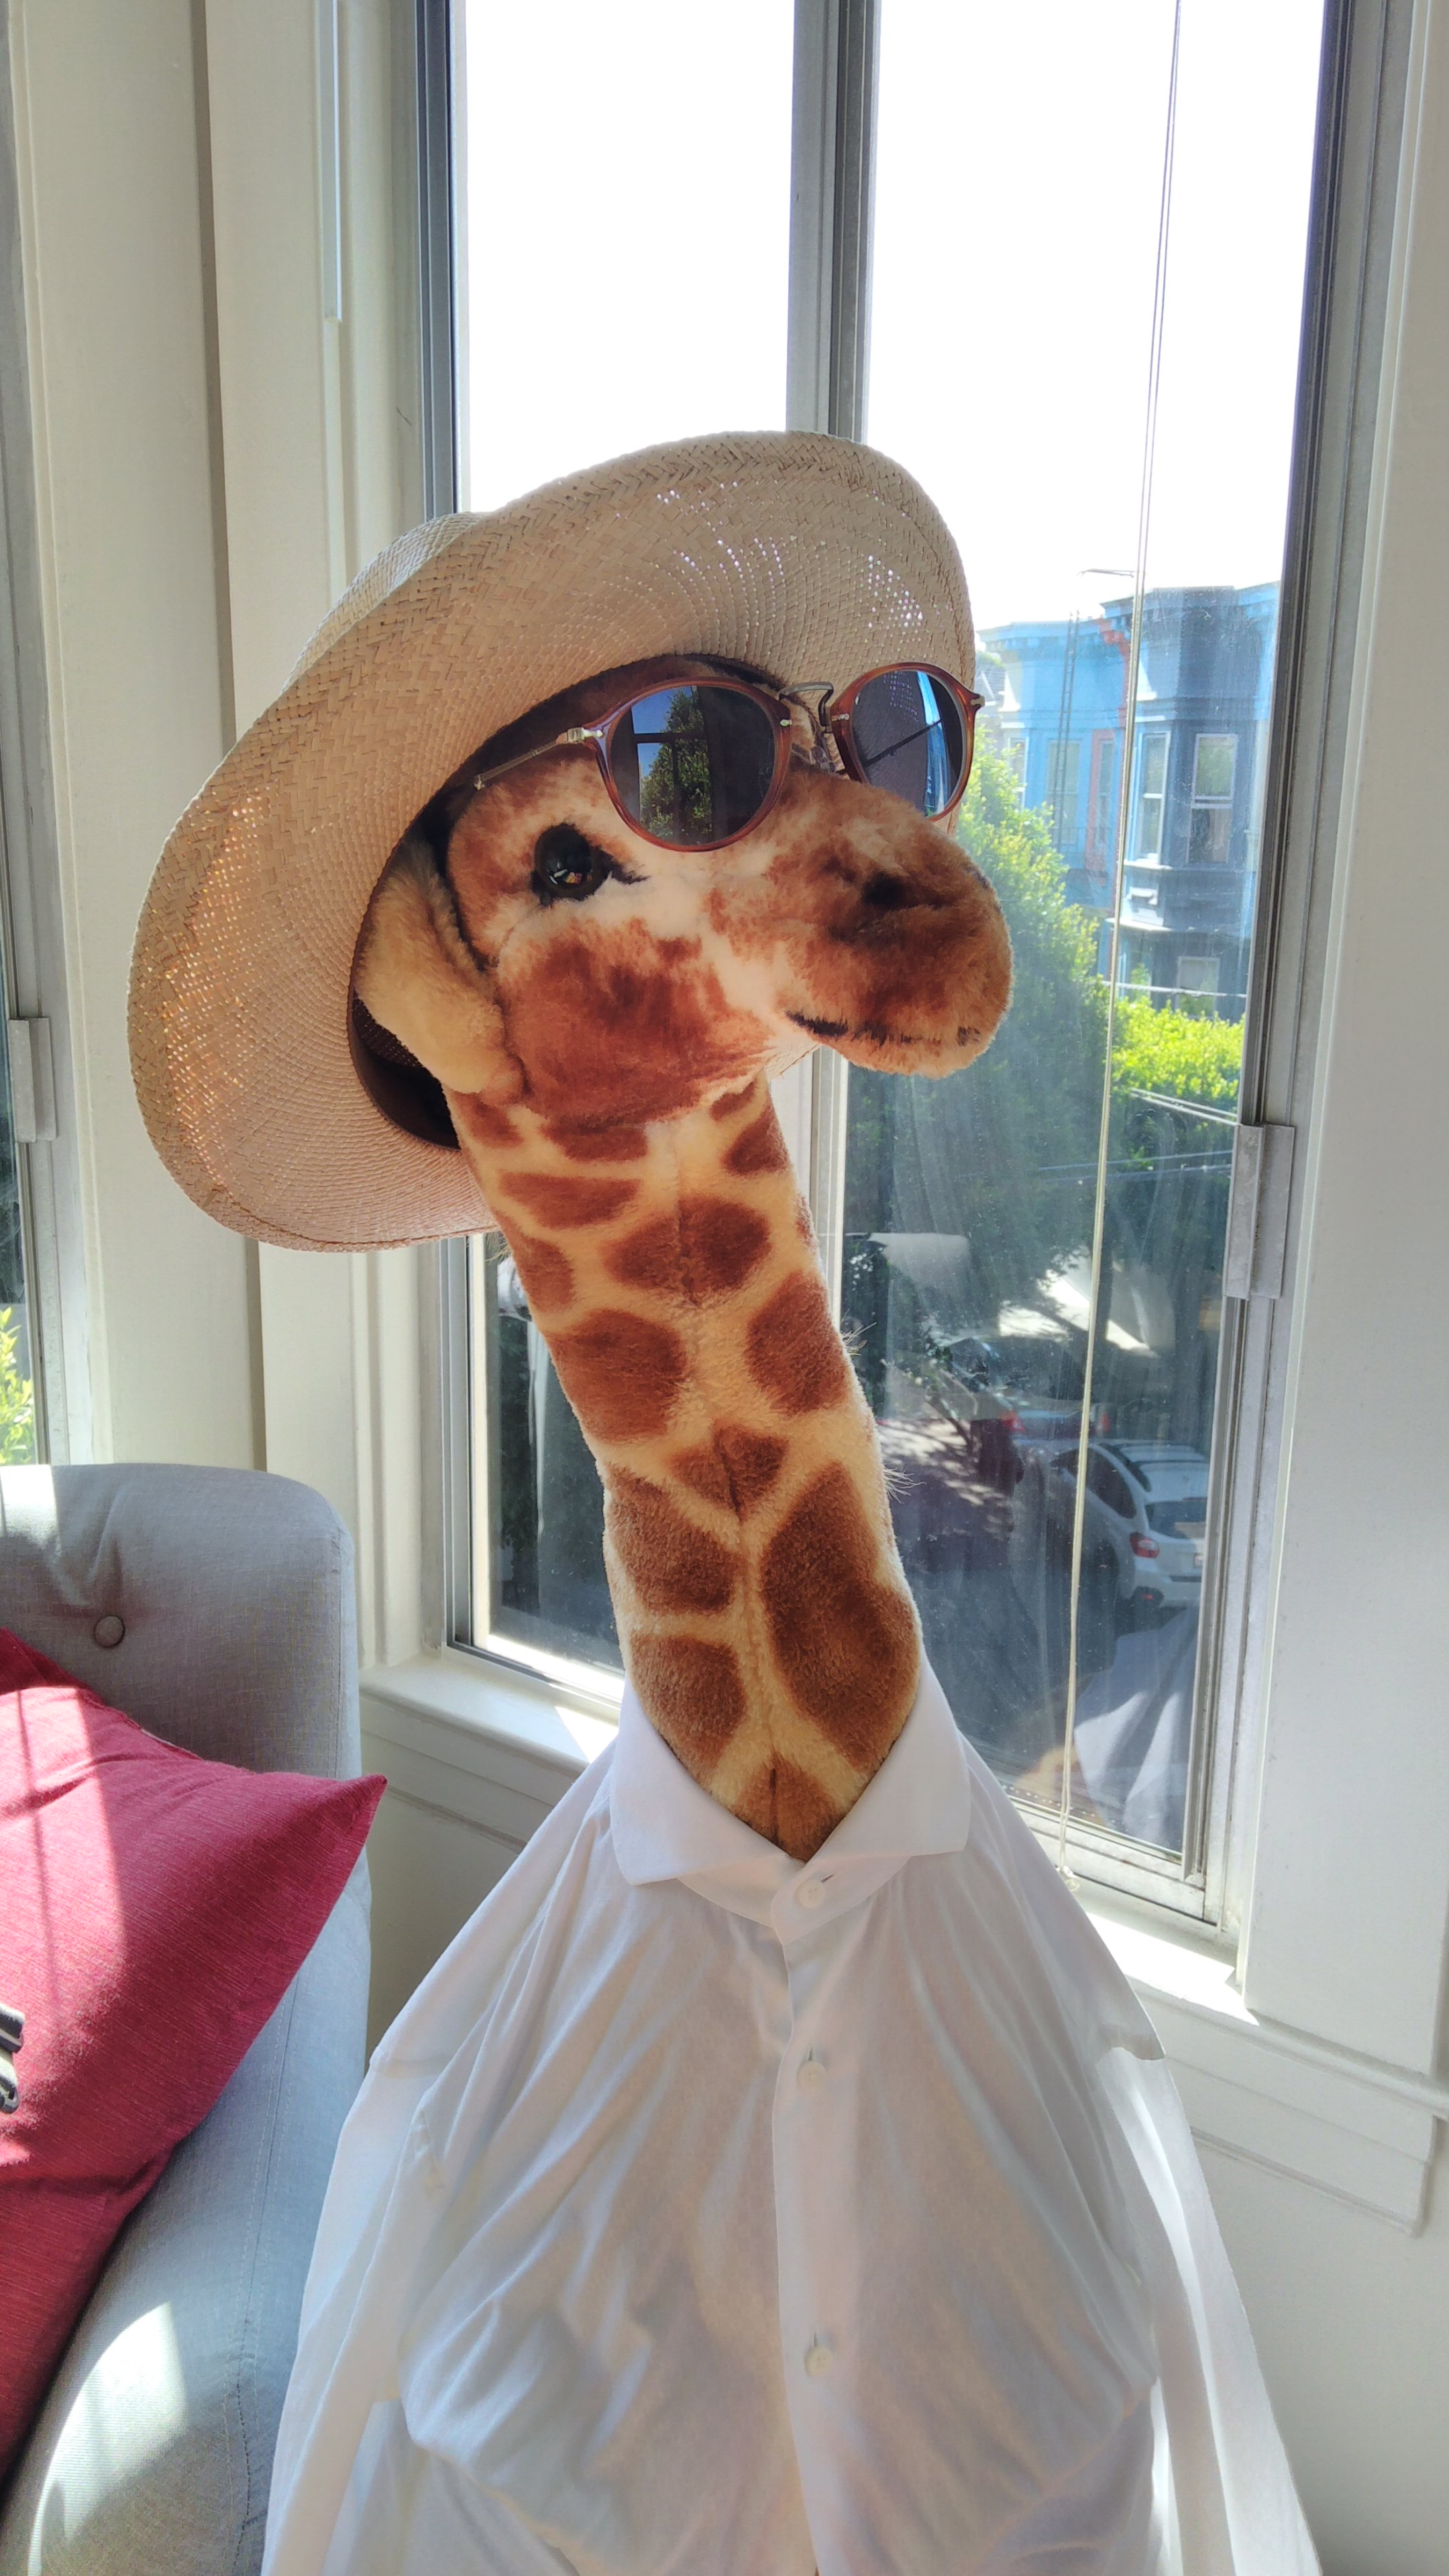
\includegraphics[width=\textwidth]{gigi.jpg}

(b) Describe what caused the bug. You can write the corrected lines as your answer below.
\begin{python}
# Put the correct code here.
\end{python}


% Please leave the pagebreak
\pagebreak
\paragraph{A5.2} (Extra space)
\end{document}

